En este capítulo se describirá el funcionamiento del algoritmo estéreo, así como también se compararán algunos métodos de reconocimiento basados en redes neuronales, para posteriormente seleccionar uno y profundizar en la forma en la que se implementó. Por último, se presentará la manera en la que detección y posicionamiento son ejecutadas mediante el paquete. 
\section{El algoritmo de visión estéreo}
En el paquete desarrollado no es obligatorio ejecutar los pasos de post-procesamiento y preprocesamiento (ver Figura \ref{stereo_pipeline}) para obtener una salida estéreo, ambos procesos se ejecutan de igual forma para cualquiera de las 4 salidas posibles, no obstante es recomendable aplicarlos si se busca obtener un mejor mapa de disparidad. Actualmente el paso de correspondencia se realiza solo con el algoritmo de correspondencia de bloques semi globales (SGBM).
\begin{figure}[H]
    \centering
    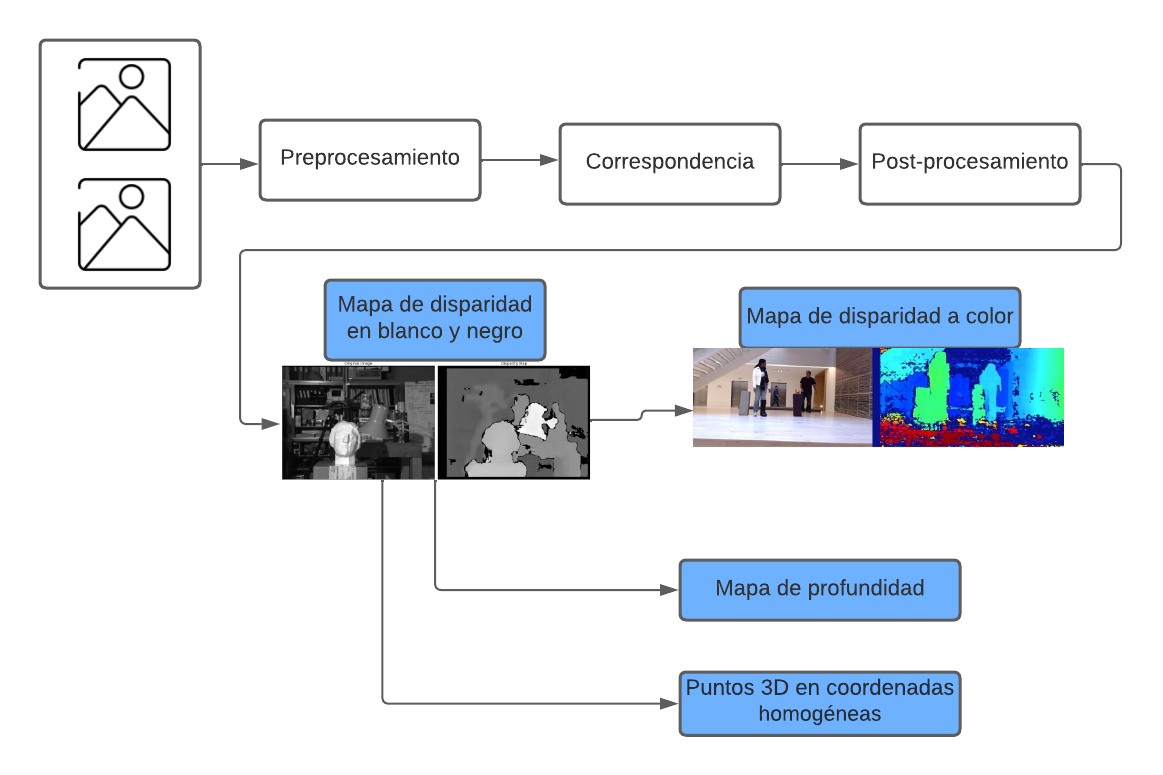
\includegraphics[scale=0.4]{Recursos/stereo_pipeline.png}
    \caption[Diagrama de flujo del mecanismo estéreo.]{Diagrama de flujo del mecanismo estéreo. {\footnotesize Fuente: El Autor}}
    \label{stereo_pipeline}
\end{figure}
\subsection{Preprocesamiento}
Consiste en efectuar las siguientes acciones:
\begin{enumerate}
    \item Se rectifican las imágenes de entrada partiendo de cámaras previamente calibradas, es decir; que de antemano se conocen los parámetros intrínsecos e extrínsecos y las matrices de translación y rotación del sistema en su conjunto. Rectificar implica calcular nuevas matrices de rotación para cada cámara de tal forma que cada plano de imagen se encuentre en una disposición paralela virtualmente hablando, lo que provoca que las líneas epipolares sean paralelas simplificando así el problema de correspondencia a una dimensión.
    \\
    \\
    En el caso de la función empleada se distinguen dos casos:
    \begin{itemize}
        \item Cuando la disposición física de las cámaras posee únicamente un desplazamiento respecto al eje de las x, por lo que las matrices de proyección (P1 y P2) poseen la siguiente forma:
        \begin{align}
           P1 = \begin{bmatrix}
            f & 0 & c_{x1} & 0\\
            0 & f & c_{y} & 0\\
            0 & 0 & 1 & 0
            \end{bmatrix}\\
            P2 = \begin{bmatrix}
             f & 0 & c_{x2} & T_{x} \cdot f\\
            0 & f & c_{y} & 0\\
            0 & 0 & 1 & 0
            \end{bmatrix}
        \end{align}
        donde $c_{x1}$ y $c_{x2}$ son los centros de proyección en $x$ de cada cámara, $c_{y}$ es el centro de proyección en $y$, $f$ es la distancia focal y $T_{x}$ es la distancia en el eje x entre las cámaras.
        \item Cuando la disposición física de las cámaras posee únicamente un desplazamiento respecto al eje de las y, por lo que las matrices de proyección (P1 y P2) serian de la siguiente forma:
        \begin{align}
           P1 = \begin{bmatrix}
            f & 0 & c_{x} & 0\\
            0 & f & c_{y1} & 0\\
            0 & 0 & 1 & 0
            \end{bmatrix}\\
            P2 = \begin{bmatrix}
             f & 0 & c_{x} & 0\\
            0 & f & c_{y2} & T_{y} \cdot f\\
            0 & 0 & 1 & 0
            \end{bmatrix}
        \end{align}
        donde $T_{y}$ es la distancia vertical entre cámaras.
    \end{itemize}
    \item Se calculan los mapas de transformación que eliminan la distorsión causada por las irregularidades del lente y a su vez guardan la configuración rectificada las imágenes de entrada.
    \item Se le aplica una convolución a cada imagen con un filtro o kernel de la siguiente forma:
    \begin{align}
        \frac{1}{256}\begin{bmatrix}
            1 & 4 & 6 & 4 & 1\\
            4 & 16 & 24 & 16 & 4\\
            6 & 24 & 36 & 24 & 6\\
            4 & 16 & 24 & 16 & 4\\
            1 & 4 & 6 & 4 & 1\\
            \end{bmatrix}
    \end{align}
   Este kernel conocido como filtro Gaussiano reduce el ancho de banda de la imagen eliminando el ruido de alta frecuencia, para posteriormente eliminar todas las filas y columnas pares de la imagen lo que provoca que la nueva imagen tenga $1/4$ de la dimensión original.
\end{enumerate}
\subsection{Correspondencia de bloques semi globales (SGBM)}
A continuacion se listan los pasos básicos de este algoritmo \cite{LearningOpenCV3}:
\begin{enumerate}
    \item Se le aplica un filtro que normaliza el brillo de la imagen para reducir las diferencias de iluminación y mejorar la textura, luego se emplea un filtro de Sobel a toda la imagen, el cual es un operador diferencial discreto que calcula una aproximación al gradiente de la función de intensidad de una imagen, esto implica que dicho filtro realza los bordes existentes.
    \item Se pre-calcula un mapa de costos de pixel C(x, y, d) que coincida con las imágenes
izquierda y derecha utilizando las métricas de Birchfield-Tomasi.
    \item Se inicializa un mapa de costos 3D S(x, y, d) con ceros.
    \item Para cada una de las tres, cuatro, cinco u ocho direcciones (r) (ver Figura \ref{cost_directions}) se calcula $S^{r}(x, y, d)$. Para minimizar el uso de memoria las primeras tres o cinco direcciones (oeste, este, norte noroeste, noreste) se
    procesan juntas, y en el caso de ocho direcciones hay un segundo paso que procesa
    las tres direcciones restantes (sur, suroeste, sureste). En el caso del algoritmo de
    tres o cinco direcciones C(x, y, d) y S(x, y, d) no se almacenan explícitamente para
    todos los píxeles; solo se almacenan las últimas tres o cuatro filas de los búfers a
    la vez.
    \begin{figure}[H]
        \centering
        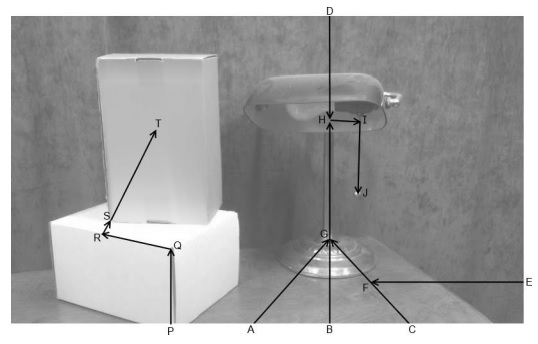
\includegraphics[scale=0.5]{Recursos/cost_directions.jpg}
        \caption[Caminos posibles para el cálculo de costos.]{Caminos posibles para el cálculo de costos. {\footnotesize Fuente: \textit{Learning OpenCV 3} \cite{LearningOpenCV3}}}
        \label{cost_directions}
    \end{figure}
    \item Una vez que S(x, y, d) está completo, se busca el valor mínimo y este es d*(x, y). Se utiliza una verificación de unicidad que calcula la diferencia entre la mejor coincidencia y la segunda mejor que se requiere para que la disparidad sea inequívoca, además se interpola el resultado para obtener una mejor respuesta
    \item Se realiza una verificación de izquierda a derecha para asegurar que las correspondencias sean consistentes y se marcan los píxeles sin coincidencias perfectas como ``disparidad no válida''.
    \item El SGBM puede tener problemas cerca de los límites de los objetos, ya que la ventana de coincidencia capta el primer plano de un lado y el fondo del otro lado, esto da como resultado una región local de grandes y pequeñas disparidades que se llaman moteado. Para evitar estas coincidencias límite, se establece un detector de manchas en una ventana de manchas, donde cada píxel se utiliza como base para la construcción de un componente conectado definido por un relleno de inundación de rango variable. El relleno de inundación de rango variable incluye un píxel vecino solo si está dentro de algún rango del píxel actual. Una vez que se calcula ese componente conectado, si es más pequeño que la ventana moteada, se considera moteado.
\end{enumerate}
El proceso anteriormente descrito requiere del ajuste de los siguientes parámetros:
\begin{itemize}
    \item \textbf{Disparidad mínima:} corresponde con el valor mínimo de disparidad buscado, comúnmente este valor es 0, pero dado que en ocasiones cuando se rectifica la imagen es desplazada hacia la izquierda o la derecha, este parámetro permite reajustar la posición de dicha imagen.
    \item \textbf{Número de disparidades:} fija el rango de las disparidades buscadas, esta ira desde el valor de la disparidad mínima sumando a este el número de disparidades, es decir; a mayor sea este valor la función de costos evaluara una mayor cantidad de píxeles, lo que implica que si se tiene un sistema con una línea base grande entre cámaras en una disposición alineada este parámetro incrementara en consecuencia.
    \item \textbf{Tamaño de bloque:} índica el tamaño de la ventana deslizante utilizada en el cálculo de coincidencias.
    \item \textbf{Disp12MaxDiff:} Dado que este algoritmo realiza el cálculo de correspondencias de la imagen izquierda a la derecha y viceversa, este valor define la diferencia mínima entre ambas correspondencias.
    \item \textbf{Rango de motas:} las motas son producidas cerca de los bordes de los objetos debido a que la ventana de correspondencia captura el plano del objeto de un lado y el fondo del otro, por lo que para eliminar estos artefactos se le aplica un filtro de motas, al cual a través de este parámetro es posible controlar que tan cerca deben encontrarse los valores de disparidad para considerarse parte del mismo bloque.
    \item \textbf{Tamaño de la ventana moteada:} es el número de píxeles por debajo del cual una mancha de disparidad se descarta como ``moteada''. 
    \item \textbf{P1 y P2:} son dos parámetros relacionados que controlan el suavizado del mapa de disparidad, es recomendable que $P2$ $>$ $P1$.
    \item \textbf{Relación de unicidad:} aplica un margen de porcentaje el cual deberá ser superado por la mejor disparidad hallada por la función de coste respecto al segundo mejor valor, en caso contrario se elegirá como ganador al segundo mejor candidato.
    \item \textbf{modo:} este controla el número de direcciones mencionadas en el paso 4.
    \item \textbf{Pre-filter cap:} su efecto es notable en el paso 1, puesto que trunca el valor de los píxeles filtrados en el rango $[-preFilterCap, preFilterCap]$. 
\end{itemize}
\subsection{Post-procesamiento}
\begin{enumerate}
    \item Al mapa de disparidad obtenido se le aplica un filtro basado en mínimos cuadrados ponderados (WLS), el cual es una generalización de los mínimos cuadrados ordinarios, dicho filtro ayuda a refinar los resultados cuando existen oclusiones y areas uniformes de las cuales no es sencillo distinguir la diferencia entre pixeles.
    \item Se redimensiona al mapa de disparidad mejorado con un filtro Laplaciano, el cual consiste en inyectar las columnas y filas pares en 0 y luego aplicar la convolución con el kernel Laplaciano, realzando así los detalles de alta frecuencia y recuperando el tamaño original.
\end{enumerate}
En esta etapa es posible modificar dos parámetros, lambda que se encarga de definir el monto de regularización durante el filtrado, haciendo que valores grandes obliguen a que los bordes del mapa de disparidad filtrados se adhieran más a los bordes de la imagen de origen. El otro sería el valor de sigma que define cuán sensible es el proceso de filtrado a los bordes de la imagen de origen. Los valores grandes pueden provocar fugas de disparidad a través de bordes de bajo contraste. Los valores pequeños pueden hacer que el filtro sea demasiado sensible al ruido y las texturas de la imagen de origen. Los valores de sigma típicos oscilan entre 0,8 y 2,0.
\subsection{Reconstrucción 3D}
A partir del mapa de disparidad de un solo canal y la matriz Q, tal que:
\begin{equation}
    Q = \begin{bmatrix}
            1 & 0 & 0 & -c_{x}\\
            0 & 1 & 0 & -c_{y}\\
            0 & 0 & 0 & f\\
            0 & 0 & -\frac{1}{T_{x}} & \frac{(c_{x} - c_{x\prime})}{T_{x}}
        \end{bmatrix}
\end{equation}
Donde $c_{x}$ y $c_{y}$ son el centro óptico de un canal y $c_{x\prime}$ es la coordenada en x del otro centro óptico, $f$ es la distancia focal y $T_{x}$ se extrae de la matriz de traslación, la importancia de esta matriz se encuentra en la siguiente expresión
\begin{equation}
    Q\begin{bmatrix}
            x\\
            y\\
            d\\
            1
        \end{bmatrix} = \begin{bmatrix}
            X\\
            Y\\
            Z\\
            W
        \end{bmatrix}
\end{equation}
Y es que dicha matriz permite convertir los mapas de disparidad en mapas de profundidad donde cada punto se encuentra en coordenadas homogéneas o simplemente hallar las coordenadas de ciertos puntos respecto al sistema estéreo.
\section{Selección de técnica de reconocimiento}\label{tecnica_recog}
Se evaluaron dos estrategias una enfocada en segmentación semántica con la arquitectura de red de DeepLab V3+ y otra basada en detección de \textit{bounding boxes} (YOLO V3), a continuación se listan las diferencias más relevantes entre ambas aproximaciones:
\begin{table}[H]
\renewcommand{\arraystretch}{1.5}
\centering
\caption{Contraste entre YOLO V3 y DeepLab V3+}
\label{deeplab_vs_yolo}
\begin{tabular}{|c|c|}
\hline
DeepLab V3+ & YoloV3 \\ \hline
\multicolumn{1}{|p{7cm}|}{La salida es una imagen donde se etiqueta cada píxel asignándole una clase.} & \multicolumn{1}{|p{7cm}|}{la salida es una matriz con las coordenadas de los \textit{bounding box}, las clases de los objetos detectados y el grado de confidencia, que no es mas que el producto entre la probabilidad de que el objeto pertenezca a la clase y el IoU.} \\ \hline
\multicolumn{1}{|p{7cm}|}{Su arquitectura se sustenta en una red \textit{encoder-decoder}} & \multicolumn{1}{|p{7cm}|}{Su arquitectura se fundamenta en una CNN del tipo ResNet} \\ \hline
\multicolumn{1}{|p{7cm}|}{Su métrica de evaluación del modelo es la mIoU, que es la IoU promedio} & \multicolumn{1}{|p{7cm}|}{Su métrica es el mAP (\textit{Mean Average Precision})} \\ \hline
\multicolumn{1}{|p{7cm}|}{Se enfoca más en la precisión que en la velocidad por lo que su tiempo de inferencia es mayor} & \multicolumn{1}{|p{7cm}|}{Alcanza un valor de precisión menor, sin embargo; su tiempo de inferencia es menor} \\ \hline
\multicolumn{1}{|p{7cm}|}{Debido a que posee un bloque ASPP es capaz de comprender de mejor forma la información contextual de objetos a diferentes escalas} & \multicolumn{1}{|p{7cm}|}{Realiza las predicciones a 3 diferentes escalas, extrayendo las \textit{features} por cada escala, similar a las redes FPN \cite{FPN} }\\ \hline
\end{tabular}
\end{table}
Al ser el objetivo final el posicionamiento de objetos junto al algoritmo estéreo mencionado en la sección previa, es menester tomar en cuenta el como se realizaría dicha acción en los dos casos:
\begin{itemize}
    \item \textbf{DeepLab V3+:} con la segmentación de la imagen de entrada se buscarían las proyecciones 3D de todos los píxeles de disparidad que pertenezcan a la clase en cuestión y posteriormente se calcula el promedio en cada coordenada, de modo que el resultado sería la distancia media con el objeto.
    \item \textbf{YOLO V3:} su cálculo es un tanto más complejo debido a que los \textit{bounding boxes} podrían contener píxeles que no correspondan con la clase dada, por lo que se ideó una forma que requiere un procesamiento extra, pero logra un resultado similar al de DeepLab V3+, esta consiste en que a cada región enmarcada por los \textit{bounding boxes} en la imagen de entrada, se le aplique un filtro gaussiano que suavice los bordes, para luego aplicar el método de umbralización de Otsu, el cual asignara como 0 a los valores de píxeles que estén por debajo de cierto umbral (el fondo del objeto detectado) y 1 al objeto en sí mismo, de modo que a los que tengan un valor de uno se les halle sus coordenadas en el plano de imagen y finalmente se proyecten al plano 3D por medio de la matriz Q y el mapa de disparidad obtenido, entonces al igual que con la segmentación se halla el promedio.
\end{itemize}
Tomando en cuenta las características mencionadas y las cualidades del hardware empleado, se eligió la red YOLO V3, principalmente porque esta posee una arquitectura que requiere una menor cantidad de iteraciones para el entrenamiento, su velocidad es mayor, lo que permite comprobar su tiempo de inferencia en local además de en Google Colab, cuenta con una versión para dispositivos móviles que es más rápida aun, a costa de la precisión y que a pesar de que requiere un par de pasos extra para posicionar un objeto sigue siendo más veloz que una red como DeepLab V3+.
\\
\\
Adicionalmente antes de implementar YOLO V3 se experimentó con la herramienta Tensorflow API model zoo que alberga una variedad de redes neuronales y entre ellas se eligió una red similar a YOLO de nombre SSD (\textit{Single shot detector}), no obstante se observó que a pesar lo útil que pueda ser la herramienta posee el problema de que para usarse depende del repositorio alojado en https://github.com/tensorflow/models.git y de la librería protobuf ambos archivos son excesivamente pesados para un paquete, puesto que esta API (\textit{Aplication Program Interface}) está diseñada para entornos virtuales con mayores capacidades como pueden ser servidores dedicados, por lo que se desechó esta posibilidad para aligerar el peso del paquete y facilitar el uso del mismo.
\section{Implementación de YOLO V3}
\subsection{Arquitectura}
Se agregaron dos tipos su versión por defecto (YOLO V3) y su versión diseñada para dispositivos móviles (YOLO V3 Tiny), la primera consta de tres partes, una para la extracción de características fundamentada en la arquitectura Darknet53 \cite{yolov3} que utiliza bloques residuales para formar una ResNet, la segunda parte que se encarga de crear las tres ramas para la detección de objetos a 3 escalas diferentes y la tercera que es similar para ambas arquitecturas y es la que entrega la matriz de predicciones. YOLO V3 Tiny se diferencia en que en lugar de usar Darknet53 se sustenta en Darknet19, la otra diferencia es que en lugar de crear 3 ramas se crean solo 2 una para las predicciones de objetos de gran tamaño y otra para los objetos de tamaño mediano. 
\subsection{Entrenamiento} 
El método que permite esta función requiere que las anotaciones introducidas se encuentren en el formato adecuado, como se pudo observar en el capítulo III esto se logra con los archivos annotations\_parser.py y annotations\_helper.py. Estos separan las anotaciones en entrenamiento, validación y en caso de ser necesario se puede separar el subconjunto de evaluación. Para entrenar también se necesita la ubicación del archivo que contenga una lista con las clases que detectara la red. Entre los hiperpárametros más importantes que el usuario puede modificar se encuentran:
\begin{itemize}
    \item \textbf{Warmup\_epochs:} este nace del hecho de que al comienzo del entrenamiento todos los hiperpárametros son típicamente aleatorios y suelen encontrarse lejos de su valor final, por esto al principio se usa una tasa de aprendizaje cercana a 0 que va creciendo linealmente bajo la expresión \eqref{warmup_lineal}
    \begin{equation}
        lr = \frac{step\_n \cdot lr\_init}{warmup\_steps}\label{warmup_lineal}
    \end{equation}
    donde $lr$ es la tasa de entrenamiento, $step\_n$ es el número de iteración el cual comienza en 1 y sube con cada iteración, lr\_init es un hiperpárametro que también controla el usuario y corresponde con la tasa de entrenamiento inicial y warmup\_steps esta dado por la expresión \eqref{warmup_steps}
    \begin{equation}
        warmup\_steps = \frac{warmup\_epochs \cdot dataset\_size}{batch\_size} \label{warmup_steps}
    \end{equation}
    En la expresión \eqref{warmup_steps} se observa donde se involucra warmup\_epochs, dataset\_size es el tamaño del conjunto de datos total y batch\_size es otro hiperpárametro que coincide con la cantidad de imágenes que se le introducen a la red en una iteración. 
    \\
    Cuando el número de la iteración supera el valor de warmup\_steps (los parámetros y métricas comienzan a converger) la función que controla la tasa de aprendizaje cambia a:
    \begin{equation}
        lr = lr\_end + \frac{lr\_init - lr\_end}{2}\cdot \left(1 + \cos\left(\frac{(step\_n - warmup\_steps)\pi}{dataset\_size - warmup\_steps}\right) \right) \label{lr_cos}
    \end{equation}
    lr\_end es la tasa final que siempre debe ser más pequeña que la inicial, cuando la ecuación \eqref{lr_cos} se activa, el $lr$ ira decayendo lentamente desde lr\_init  hasta lr\_end hasta que se acabe el entrenamiento.
    \item \textbf{\textit{epochs}:} para entender su valor, es menester comprender el ciclo de la rutina de entrenamiento, la cual consiste en:
    \begin{enumerate}
        \item Introducir a la red un lote de imágenes de tamaño igual al batch\_size.
        \item Predecir o inferir la matriz de salida.
        \item Calcular el error con la función de coste el cual está compuesto por 3 errores distintos:
        \begin{enumerate}
            \item El error de clasificación o error de probabilidad
            \item El error de confianza que representa la existencia de un objeto en un \textit{bounding box}.
            \item El error dado por el IoU, en este caso se utilizó la métrica GIoU que es una forma generalizada del IoU.
        \end{enumerate}
        \item Aplicar el algoritmo del descenso al gradiente con el optimizador de Adam.
        \item Ajustar la tasa de aprendizaje o \textit{learning rate} con la metodología \textit{warmup} previamente descrita.
        \item Repetir todos los pasos previos hasta introducir todos los datos de entrenamiento.
        \item Realizar los pasos 1, 2 y 3 para todo el conjunto de validación. 
        \item Guardar los pesos y parámetros del modelo.
    \end{enumerate}
    Las instrucciones mencionadas comprenden 1 \textit{epoch}, por lo que para entrenar una red estos pasos se deben ejecutar una cantidad $n$ de \textit{epochs} o épocas.
\end{itemize}
\subsection{Recuperación de pesos}
Dado que los pesos de una red conservan el entrenamiento por el que paso el modelo, se crearon dos formas para tomar los pesos de un archivo con un mismo método, existe la opción de tomarlos de un archivo conocido como \textit{checkpoint} que es generado por la red al momento del entrenamiento en cada época o incluso utilizar los pesos originales de la red YOLO V3 entrenada con el conjunto de datos COCO el cual cuenta con 80 clases diferentes a detectar, crear esta opción fue necesario debido a que los pesos originales poseen un formato .weights el cual no es compatible con los métodos propios de Tensorflow para su recuperación.
\subsection{Inferencia}
Como se mencionó en el capítulo III existen 4 formas de inferencia compatibles con cualquier modelo de detección en el archivo detection\_mode.py, sin embargo el algoritmo que realiza esta tarea en líneas generales sigue los procesos de la Figura \ref{inference_diagram}, entonces la inferencia consiste en 4 etapas, el preprocesamiento que reduce la imagen a unas dimensiones compatibles con la arquitectura de la red, la predicción que entrega una matriz de dimensiones $n$ $x$ $6$, el post-procesamiento que redimensiona los \textit{bounding boxes} y la imagen al tamaño original, además de aplicar el algoritmo NMS y por último se dibujan en la imagen los \textit{bounding boxes} con la clase de cada objeto y el grado de confidencia.
\begin{figure}[H]
    \centering
    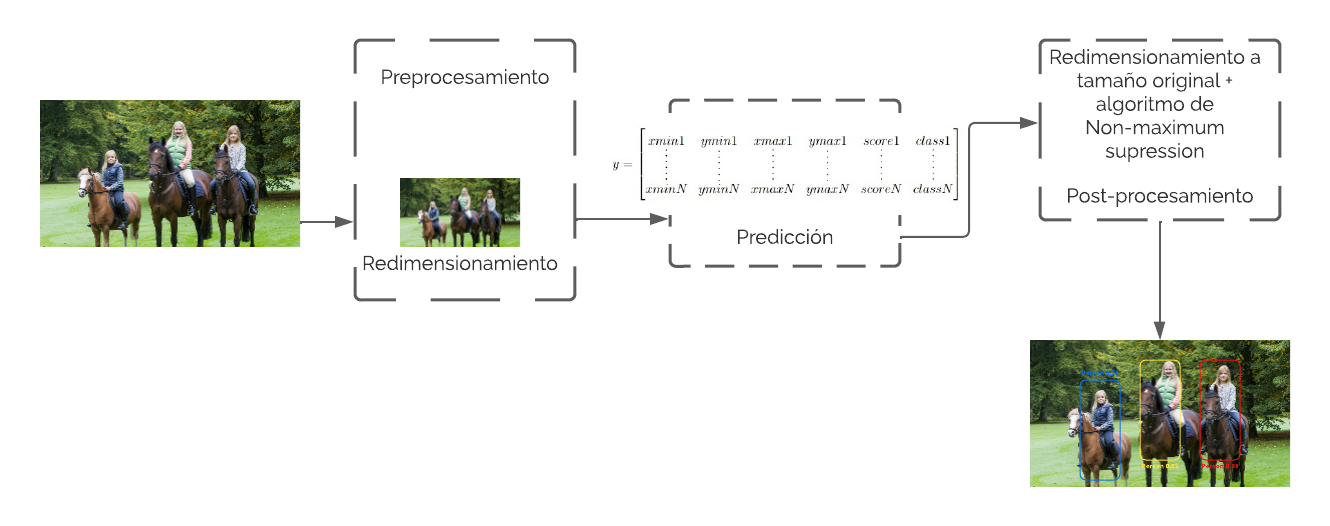
\includegraphics[scale=0.6]{Recursos/inference_cycle.png}
    \caption[Ciclo de inferencia.]{Ciclo de inferencia. {\footnotesize Fuente: El Autor}}
    \label{inference_diagram}
\end{figure}
\subsection{Evaluación}
Se utilizó la métrica mAP (\textit{Mean Average Precision}) para evaluar la precisión de la red, esta se fundamenta en la IoU y los siguientes conceptos:
\begin{itemize}
    \item \textbf{Precisión:} mide cuán preciso son las inferencias y se calcula con la siguiente ecuación:
    \begin{equation}
        prec = \frac{TP}{TP + FP} = \frac{TP}{Casos\; positivos}
    \end{equation}
    donde TP (\textit{True Positive}) es la cantidad de predicciones cuyo resultado coincide con el \textit{ground truth} y la clase verdadera, FP (\textit{False Positive}) son las predicciones cuyo resultado tiene una probabilidad mayor a un umbral definido por el usuario, pero que no coincide con el \textit{ground truth} y la clase.
    \item \textbf{\textit{Recall}:} mide que tan bueno es el detector para hallar todos los positivos, se mide con la siguiente expresión:
    \begin{equation}
        rec = \frac{TP}{TP + FN} = \frac{TP}{Casos Totales}
    \end{equation}
    FN (\textit{False Negative}): son las predicciones que no superan el umbral definido, pero que aun así coinciden con el resultado real.
\end{itemize}
El valor de AP (\textit{Average Precision}) esta definido como:
\begin{equation}
    AP = \int_{0}^{1} p(r)dr
\end{equation}
donde $p(r)$ es el área bajo la curva precisión vs. \textit{recall} que se forma con todos los datos de evaluación, AP es calculado para cada clase por separado, de tal modo que mAP es el promedio formado por todas las clases del modelo. 
\section{Posicionamiento de objetos}
Al ser este el objetivo final del paquete la clase \textbf{VisionSystem} abarca la rutina de cálculo de disparidad más detección para imágenes, \textit{streaming} y vídeo. Asumiendo que previamente se realizó la calibración de las cámaras, se obtuvieron mapas que rectifican las imágenes izquierda y derecha del sistema estéreo y se hallaron los parámetros adecuados para el algoritmo SGBM. Adicionalmente requiere que el modelo de AA haya sido entrenado previamente para obtener un resultado satisfactorio.
\\
\\
Con todos estos elementos en la Figura \ref{vision_system_cycle} se puede observar como la imagen de la izquierda es sobre escrita para obtener el resultado final, de igual forma el filtro WLS (mínimos cuadrados ponderados) que corresponde con el post-procesamiento estéreo utiliza como referencia el mapa de disparidad izquierdo, por lo que el mapa refinado corresponde con la imagen de la izquierda y el cálculo de distancia sigue la misma metodología descrita en la sección \ref{tecnica_recog}.
\begin{figure}[H]
    \centering
    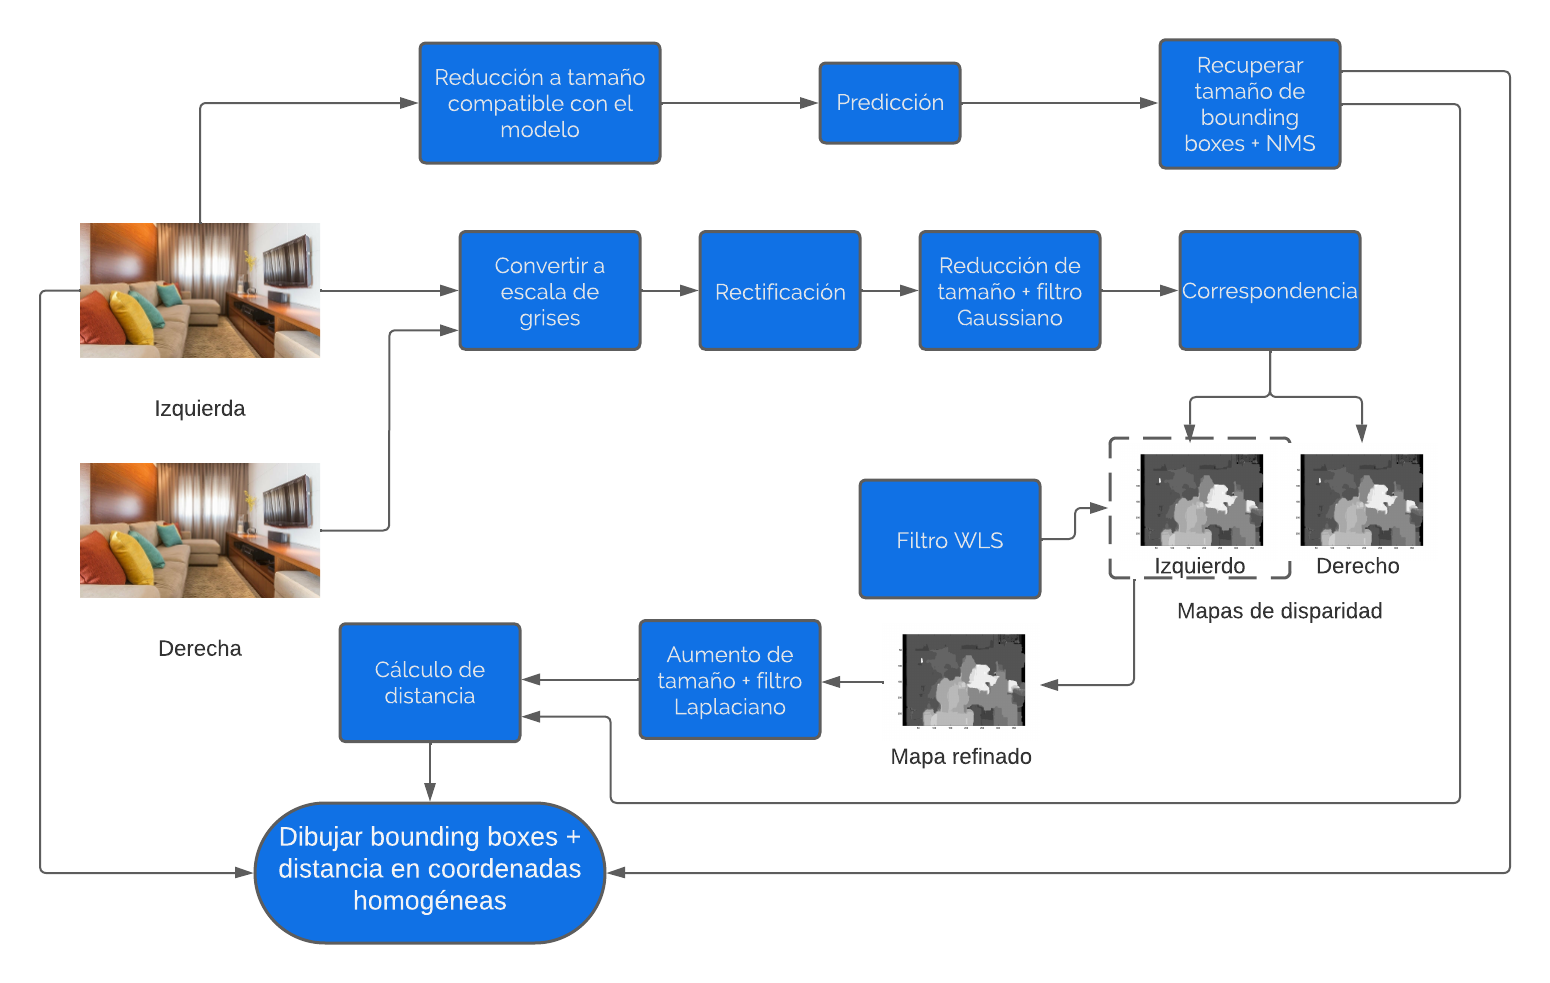
\includegraphics[scale=0.6]{Recursos/vision_system_cycle.png}
    \caption[Diagrama para el posicionamiento con visión estéreo y YOLO V3.]{Diagrama para el posicionamiento con visión estéreo y YOLO V3. {\footnotesize Fuente: El Autor}}
    \label{vision_system_cycle}
\end{figure}